\documentclass[10pt,letterpaper]{article}
\usepackage[left=1.8cm, right=1.8cm, top=1cm]{geometry}
\usepackage[utf8]{inputenc}
\usepackage[T1]{fontenc}
\usepackage[spanish]{babel}
\usepackage{amsmath}
\usepackage{amsfonts}
\usepackage{amssymb}
\usepackage{graphicx}
\usepackage{subfigure}
\usepackage{steinmetz}
\usepackage{float}
%\usepackage{circuitikz}

\author{Clase Práctica $\#$5}
\title{Electrónica I}
\date{Análisis de circuitos en el dominio de $s$. Potencia.}

\renewcommand{\sin}{\sen}
\begin{document}
	\maketitle
	
Bibliografía: Análisis de circuitos en ingeniería. Hayt \textit{et al.} 8va ed. Capítulos 10, 11, 14 y 15.
\\
1- Respecto al circuito representado en la figura:

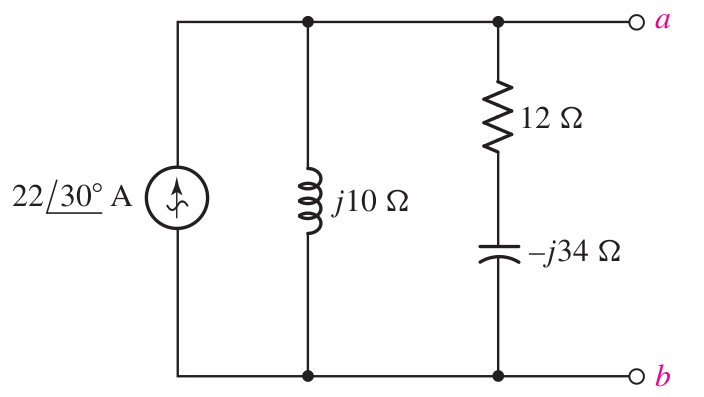
\includegraphics[scale=0.35]{c1} 

a) Calcule el equivalente de Thévenin visto desde las terminales marcadas $a$ y $b$.

b) Determine el equivalente de Norton visto desde las terminales marcadas $a$ y $b$.

c) Calcule la corriente que fluye de $a$ a $b$ si una impedancia de $(7-2j)\:\Omega$ está conectada entre dichas terminales. \\

2- Determine la corriente $i(t)$ del circuito de la figura.

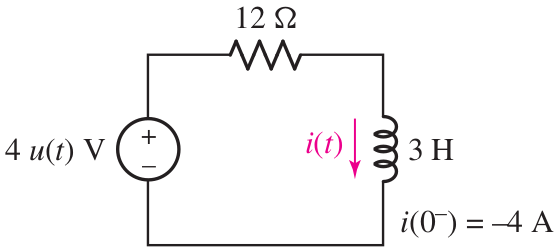
\includegraphics[scale=0.45]{c2} \\

3- Calcule la tensión $v_x$ en el circuito de la figura utilizando las técnicas del análisis nodal. \textbf{(EJEMPLO 15.4)}

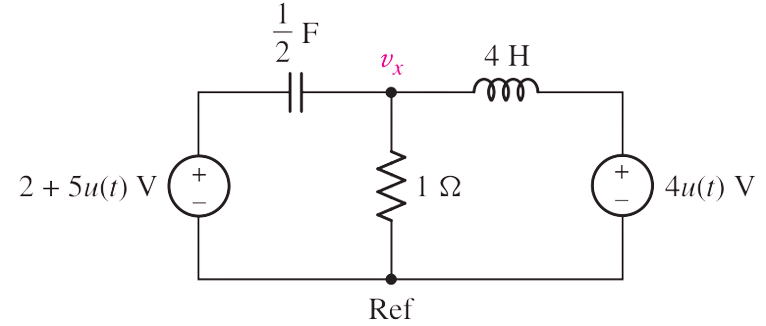
\includegraphics[scale=0.45]{c3} \\

4- Con referencia al circuito de dos mallas representado en la figura, determine la potencia promedio absorbida por cada elemento pasivo y la potencia promedio suministrada por cada fuente, y verifique que la potencia promedio total suministrada = potencia promedio total absorbida.

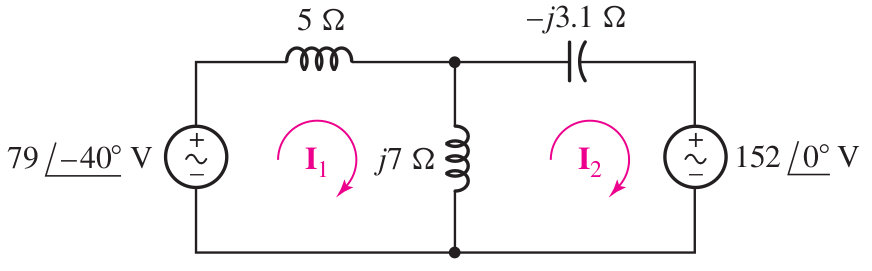
\includegraphics[scale=0.4]{c_p1}

5- Con referencia al circuito de la figura, determine si un valor puramente real de R puede dar por resultado tensiones rms iguales entre las terminales del inductor de $14 \mathrm{mH}$ y la resistencia R. Si es así, calcule R y la tensión rms entre sus terminales; si no, explique por qué no.

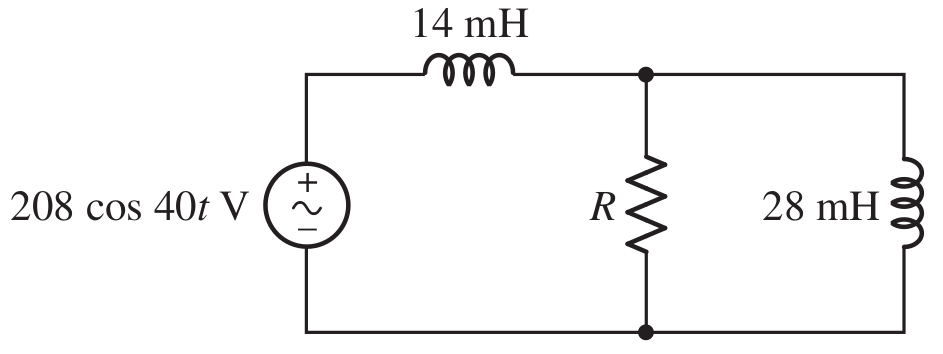
\includegraphics[scale=0.3]{c_p2}

6- Calcule la potencia compleja suministrada a cada componente pasivo del circuito que se muestra en la figura, y determine el factor de potencia de la fuente.

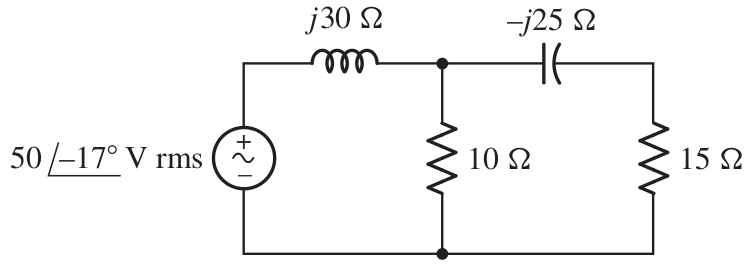
\includegraphics[scale=0.45]{c_p3}

a) Reemplace la resistencia de 10 $\Omega$ en el circuito de la figura por un inductor de $200 \mathrm{mH}$, suponga una frecuencia de operación de 10 rad/s y calcule: el FP de la fuente, la potencia aparente suministrada por la fuente y la potencia reactiva suministrada por la fuente.
\end{document}